\documentclass[a4paper]{article}

\usepackage[T1]{fontenc}
\usepackage[lf]{Baskervaldx} % lining figures
\usepackage[bigdelims,vvarbb]{newtxmath} % math italic letters from Nimbus Roman
\usepackage[cal=boondoxo]{mathalfa} % mathcal from STIX, unslanted a bit
\renewcommand*\oldstylenums[1]{\textosf{#1}}

\usepackage{background}
\usepackage[margin=0cm]{geometry}
\usetikzlibrary{calc}

\backgroundsetup{scale = 1, pages=some, angle = 0, opacity = 1, color=black, contents = {
\includegraphics[width = \paperwidth, height = \paperheight] {bg-1.pdf}}}
\begin{document}
    \sffamily
    \noindent 
\begin{tikzpicture}[yscale=-1, remember picture, overlay] \end{tikzpicture}
    

    \pagebreak

    \begin{tikzpicture}[yscale=-1, remember picture, overlay]
        % \useasboundingbox (2.52,6.67) rectangle (18.47,12.85);
        % \fill[fill=white, opacity=0.9] (25mm,63mm) rectangle ++(160mm,62mm);

        \coordinate (A) at (19mm, 128.0mm);
        \coordinate (B) at ($(A)+(0mm,5mm)$);
        \coordinate (C) at (19mm,212mm);

        \path (A) node[anchor=west,fill=white,text width=120mm,text height=2.5mm,inner xsep=0mm,inner ysep=1mm]{<<<$name>>>};
        \path (B) node[anchor=west,fill=white,text width=120mm,text height=2.5mm,inner xsep=0mm,inner ysep=1mm]{<<<$secondLine>>>};
        \path (C) node[anchor=west,fill=white,text width=120mm,text height=2.5mm,inner xsep=0mm,inner ysep=1mm]{Neuss, <<<$now>>>};
    \end{tikzpicture}

    \backgroundsetup{scale = 1, pages=some, angle = 0, opacity = 1, color=black, contents = {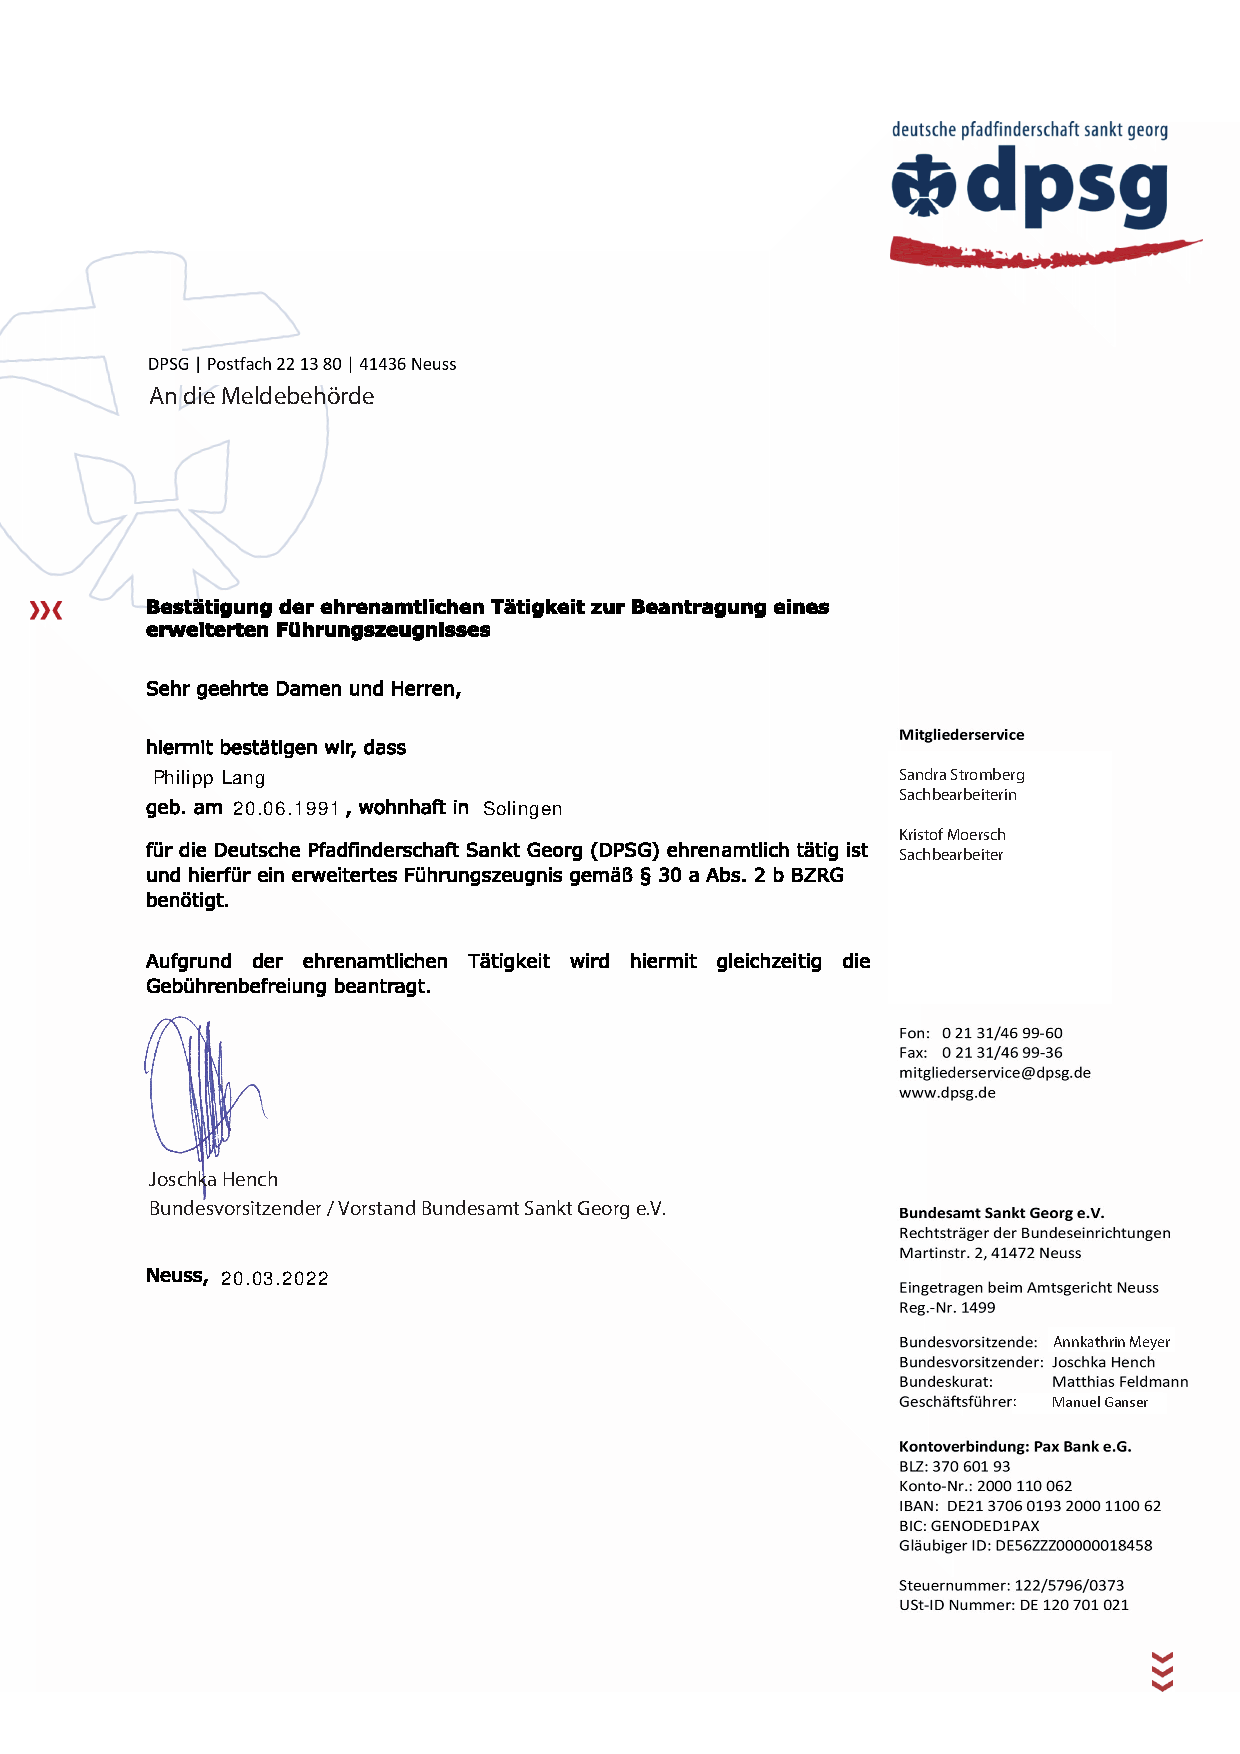
\includegraphics[width = \paperwidth, height = \paperheight] {bg-2.pdf}}}

    \pagebreak
    \backgroundsetup{scale = 1, pages=some, angle = 0, opacity = 1, color=black, contents = {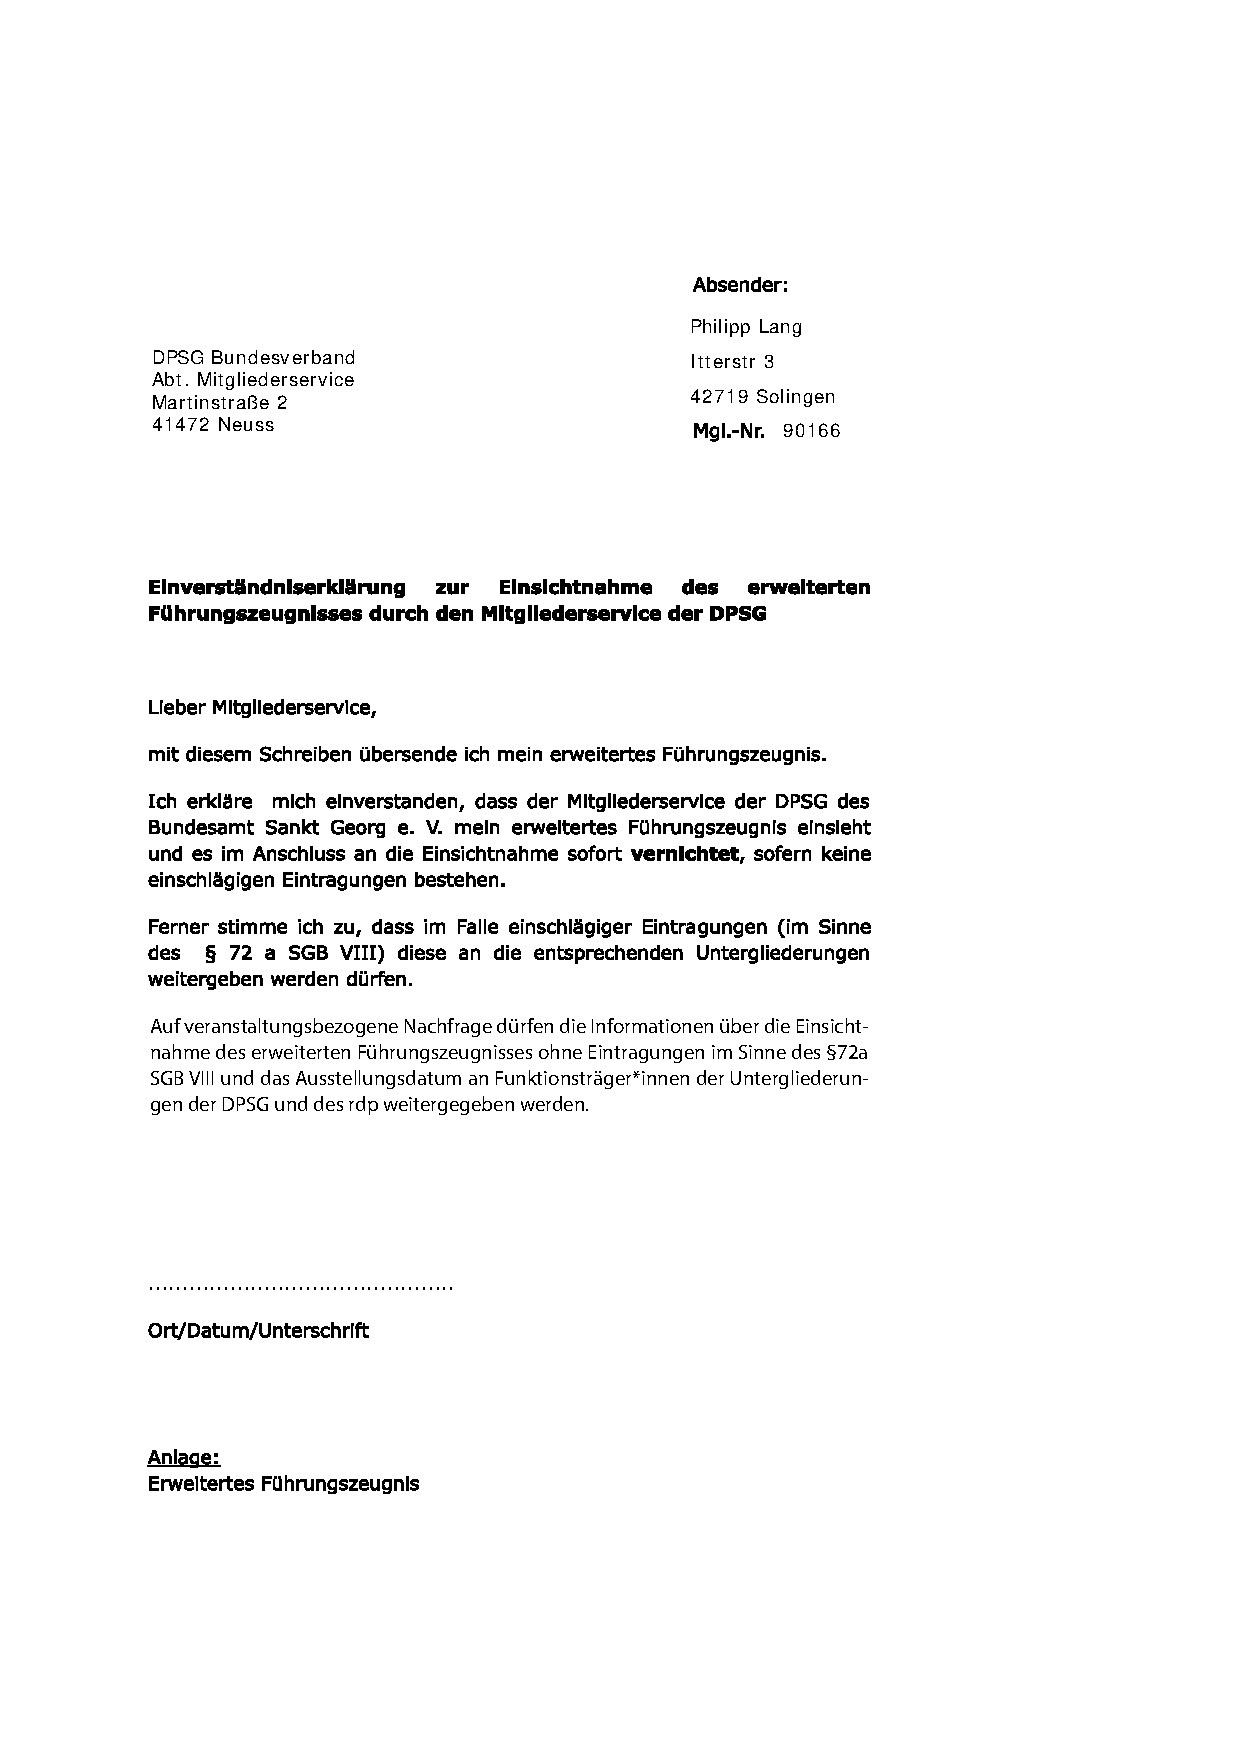
\includegraphics[width = \paperwidth, height = \paperheight] {bg-3.pdf}}}

    \begin{tikzpicture}[yscale=-1, remember picture, overlay]
        % \useasboundingbox (2.52,6.67) rectangle (18.47,12.85);
        % \fill[fill=white, opacity=0.9] (25mm,63mm) rectangle ++(160mm,62mm);

        \node[anchor=north west,fill=white,text width=80mm,minimum height=30mm,inner sep=1mm] at (110mm, 42.0mm) {Absender: \vspace{2mm} \\ <<<implode(' \\\\ ', $sender->values())>>>};
    \end{tikzpicture}

\end{document}


